\chapter{Control óptimo de sistemas nolineales}

\section{Planteamiento (caso general)}

Dado un sistema dinámico:

\begin{align*}
    \dot{x}(t)=f\big( x(t),u(t),t\big) 
\end{align*}

Problema es encontrar $u(t)$, para llevar el estado $x(t)$ hasta $x(t_1)$, para un tiempo finito $t\in[t_0,t_1]$, tal que se cumpla la siguiente condición, donde $J(u)$ es el funcional de desempeño:

\begin{align*}
    J(u) = \int_{t_0}^{t_1} \mathcal{L} \big( x(t), u(t), t \big) dt + m \big( x(t_1) \big)
\end{align*}

\begin{itemize}
    \item $\int_{t_0}^{t_1} \mathcal{L} \big(x(t),u(t),t\big)dt$: ``Costo de viaje'' (running cost)
    \item $m \big( x(t_1) \big)$: costo terminal
\end{itemize}

El problema de control óptimo se define como:

\begin{align*}
    u^\star = \arg \min_{u_{[t_0,t_1]}} J(u)
\end{align*}

Se define la \textcolor{red}{función de valor V} como el mínimo costo posible para la trayectoria del sistema dinámico para todos los controles posibles $u_{[t_0,t_1]}$:

\begin{align*}
    V(x_0,t_0) = \min_{u_{[t_0,t_1]}} J(u) = \min_{u_{[t_0,t_1]}} \Big\{\int_{t_0}^{t_1} \mathcal{L} \big(x(t),u(t),t\big)dt+m\big(x(t_1)\big)  \Big\}
\end{align*}

\section{Principio de Optimalidad}

Para cada $t\in[t_0,t_1)$ y $x\in\mathbb{R}^n$, y para $\Delta t\in[0,t_1-t)$, la función de valor $V(x,t)$ satisface la relación: 

\begin{align*}
    V(x,t) = \min_{u_{[t,t+\Delta t]}} \Big\{ \int_t^{t+\Delta t} \mathcal{L}\big(x(s),u(s),s\big)ds+V\big(x(t+\Delta t),t+\Delta t\big)\Big\}
\end{align*}

\begin{itemize}
    \item $\int_t^{t+\Delta t} l\big(x(s),u(s),s\big)ds$: costo asociado al intervalo $[t+\Delta t]$
    \item $V\big(x(t+\Delta t),t+\Delta t\big)$: ``costo a seguir'' mínimo partiendo en $x(t+\Delta t)$ y $t+\Delta t$ $\Longrightarrow$ costo asociado al intervalo $[t+\Delta t,t_1]$
\end{itemize}

Entonces, el principio de optimalidad (de Bellman) estable que para que una solución completa sea la mejor (óptima), cada parte de esa solución también tiene que ser la mejor posible.

\underline{Intuición}:

\begin{figure}[H]
    \centering
    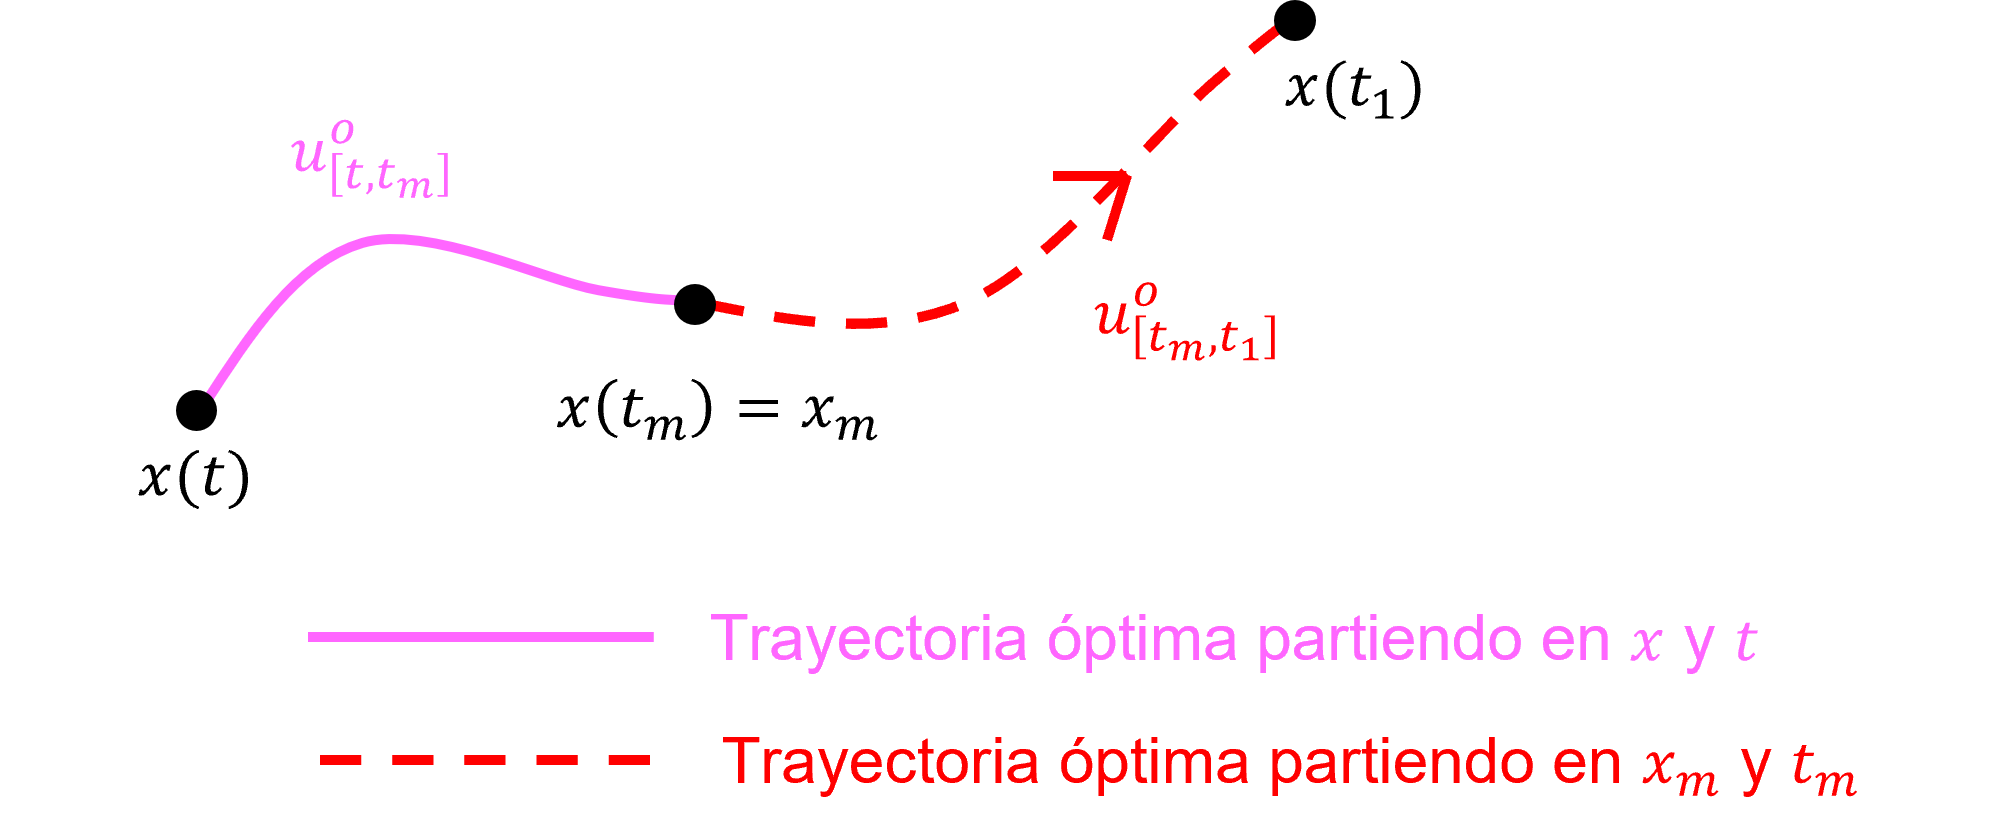
\includegraphics[scale=0.7]{Figuras/optimalidad.png}
\end{figure}

\section{Ecuación HJB (Hamilton-Jacobi-Bellman)}

Esta ecuación resuelve $V(x,t)$ y se obtiene de la siguiente forma:

\begin{enumerate}
    \item Principio de Optimalidad
    \item Realizar una expansión de Taylor de $V(x+\Delta x,t+\Delta t)$ con respecto a $V(x,t)$
    \item Combinar 1. y 2. y dividir por $\Delta t$
    \item Calcular límite para $\Delta t\to 0$
\end{enumerate}

\begin{align*}
    \text{Ec. HJB: } \quad -V_t(x,t) = \min_{u \in \mathcal{U}} \left\{ \mathcal{L}(x,u,t) + \left( \nabla_x  V(x,t) \right)^T f(x,u,t) \right\}
\end{align*}

donde $V_t=\frac{\partial V}{\partial t}$, $\nabla_x V=\frac{\partial V}{\partial x}$ \\

\par Notar que la ecuación HJB es una ec. diferencial parcial. Por lo tanto, para resolver necesitamos condiciones de borde:

\begin{align*}
    V\big(x(t_1),t_1\big)=m\big(x(t_1)\big)
\end{align*}

\underline{Definición}: Hamiltoniano

\begin{align*}
    \mathcal{H}(x,p,u,t) = \mathcal{L}(x,u,t) + p^T(x,t) f(x,u,t)
\end{align*}

donde $\mathcal{H}$ es el Hamiltoneano; $\mathcal{L}$ es el Lagrangiano; $p = \nabla_x V$ es la penalización de Lagrange; y $f$ es la dinámica del sistema.\\

\par Entonces, la ex. HJB se reduce a:

\begin{align*}
    -V_t(x,t)=\min_{u \in \mathcal{U}} \mathcal{H}(x,p,u,t)
\end{align*}

Con estas herramientas, formulamos el siguiente algoritmo para diseñar controladores óptimos:

\begin{enumerate}
    \item Construir el Hamiltoniano
    \item Construir la ec. HJB
    \item Buscar $u^\star = \arg \min_u \mathcal{H}(x,p,u,t)$
    \item Substituir $u^\star$ en la expresión HJB
    \begin{align*}
        -V_t = \mathcal{H}(x,p,u^\star,t)
    \end{align*}
    \item Resolver la ec. dif. parcial para determinar $u^\star$
\end{enumerate}

\section{Ejemplo Control LQR}

Sea el sistema LTI:

\begin{align*}
    \dot{x} = f(x,u) = A x + B u
\end{align*}

y el funcional de desempeño:

\begin{align*}
    J(u) =\int_{t_0}^{t_f} \left[ x^T Q x + u^T R u \right] dt + x^T(t_f) Q_f x(t_f)
\end{align*}

Requisitos: $Q$, $R$, $M$ son matrices definidas positivas y simétricas.\\

\par Utilizando el algoritmo para resolver la ec. HJB:

\begin{enumerate}
    \item[1.] Hamiltoniano:
    \begin{align*}
        \mathcal{H}(x,u,V_x,t) = x^T Q x + u^T R u + V^T_x \left( A x + B u \right)
    \end{align*}
    \item[3.] Buscar $u^\star$: $u^\star = \arg \min_u \mathcal{H}(x,u,V_x,t)$
    \begin{align*}
        \Longrightarrow \frac{\partial \mathcal{H}}{\partial u} = 0 \Longrightarrow \frac{\partial}{\partial u}\left[ x^T Q x + u^T R u + V_x^T \left( A x + B u \right) \right] = 0\\
        \Longrightarrow 2 R u + B^T V_x = 0\\
        \Longrightarrow u^\star = -\frac{1}{2} R^{-1} B^T V_x(x,t)
    \end{align*}
    \item[2. y 4.] \begin{align*}
        -V_t(x,t) &= \mathcal{H}(x,u^\star,V_t,t)\\
        \Longrightarrow -V_t &= x^T Q x + (u^\star)^T R u^\star + V_x^T \left(A x + B u^\star\right)
    \end{align*} 
    \begin{align}
        \Longrightarrow -V_t &= x^T Q x - \frac{1}{4} V_x^T B R^{-1} B^T V_x + V_x^T A x
    \end{align}
\end{enumerate}

Suponga que: $V(x,t) = x^T P(t) x$, $P(t) \in \mathbb{R}^{n \times n}$, $P^T (t)=P(t)$, $P(t) \succ 0$

\begin{align*}
    V_t &= x^T \dot{P}(t) x\\
    V_x &= 2 P(t) x
\end{align*}

Sustituyendo en (12):

\begin{align*}
    -x^T \dot{P}x &= x^T Q x-\frac{1}{4} \left( 2 P x \right)^T B R^{-1} B^T \left( 2 P x \right) + \left( 2 P x \right)^T Ax\\
    \Longrightarrow -x^T \dot{P} x &= x^T \left[Q + PA + A^T P - P^T B R^{-1} B^T P \right]x\\
    \Longrightarrow -\dot{P} &= Q + P A +A^T P -P^T BR^{-1}B^T P \quad \text{(Ecuación de Riccati)}
\end{align*}

Para resolver la ecuación (diferencial) de Ricatti, es necesaria una condición inicial (o final). En estos casos, se ocupa el costo terminal para obtener $P(t_f) = Q_f$, y con este valor hacer la integración numérica de la EDO hacia atrás (``\emph{backwards integration}''), hasta obtener $P(t)$.

Sea el cambio de variable $\tau = t_f - t, \tau \in [0, t_f-t_0]$:

\begin{align}
    \frac{dP}{dt} = \frac{dP}{d\tau} \frac{d\tau}{dt} = -\frac{dP}{d\tau}
\end{align}

Entonces:

\begin{align*}
   \dot{P}(\tau) &= Q + P(\tau) A +A^T P(\tau) - P(\tau)^T B R^{-1} B^T P(\tau), \quad \forall \tau \in [0,t_f - t_0] \\
   P(0) &= Q_f
\end{align*}

Resuelto $P(t)$, se calcula la ganancia del controlador:

\begin{align*}
    V(x,t) &= x^T P(t)x \\
    V_x(x,t) &= 2 P(t) x\\
    \Longrightarrow u^\star &= \frac{1}{2} R^{-1} B^T V_x(x,t) = -\frac{1}{2} R^{-1} B^T \left( 2 P(t) x \right)\\
    u^\star &= - R^{-1} B^T P(t) x\\
    u^\star &= -K(t) x
\end{align*}

donde $K(t) = R^{-1} B^T P(t) \Longrightarrow$ Control óptimo LQR de horizonte finito (gains variable en el tiempo)

% \begin{figure}[H]
%     \centering
%     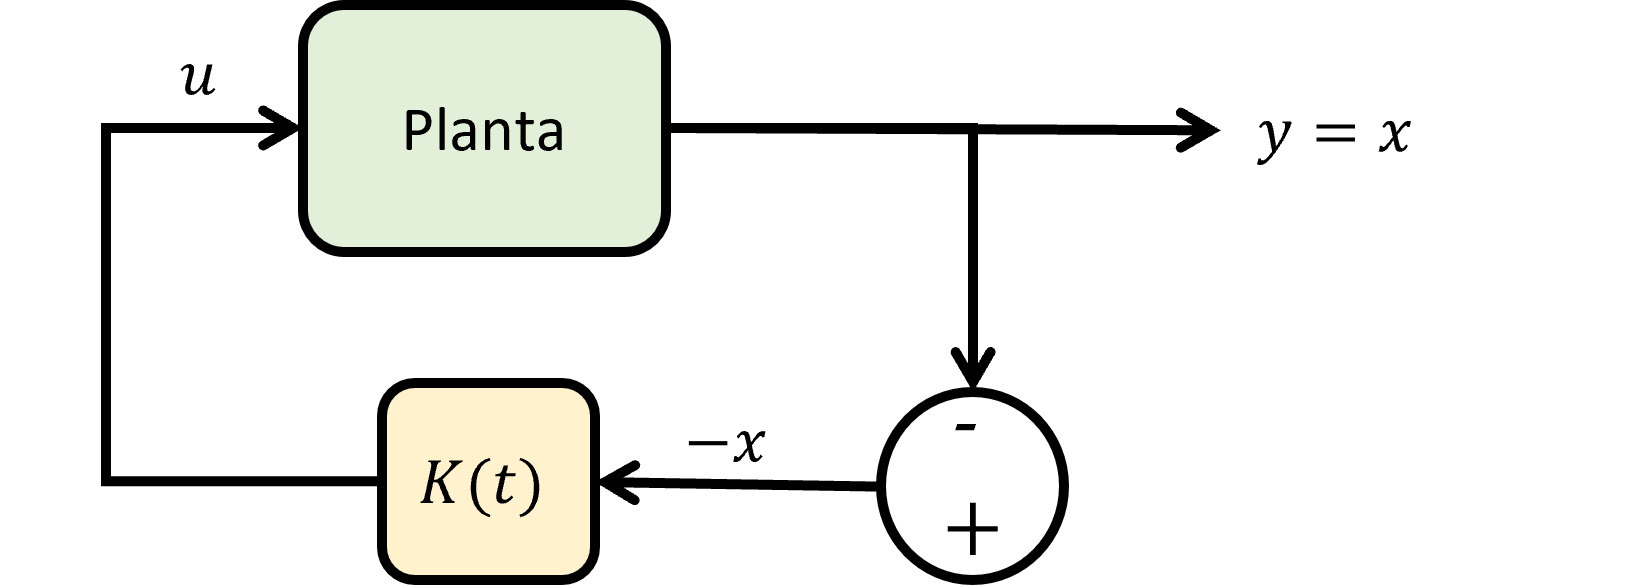
\includegraphics[scale=0.7]{Figuras/LQR.png}
% \end{figure}

% \section{Control LQR de horizonte infinito}
% Dado el sistema LTI: 
% \begin{align*}
%     \dot{x}=Ax+Bu
% \end{align*}
% Asumiendo que el sistema es:
% \begin{itemize}
%     \item estable y controlable, o
%     \item inestable, pero los estados inestables son controlables $\Longrightarrow$ estados estabilizables.
% \end{itemize}

% El problema de control óptimo LQR en horizonte infinito minimiza el siguiente funcional:
% \begin{align*}
%     J(u) = \lim_{t_1\to \infty} \left[\int_0^{t_1}(x^T Qx+u^T Ru)dt \right]
% \end{align*}
% \underline{Nota}: En este caso, el costo terminal se asume igual a 0.\\
% \par Según la lección anterior:
% \begin{align*}
%     V^{t_1}(x,t)=x^T P(t,t_1)x \quad \text{: Función de valor para horizonte finito ``$t_1$''}
% \end{align*}

% Para resolver $P(t,t_1)$, utilizamos la DRE (Differential Riccati Equation):
% \begin{align*}
%     -\dot{P}=Q+PA+A^T P-P^T BR^{-1}B^T P
% \end{align*}
% Con condiciones de borde: $P(t_1,t_1)=m(x(t_1))=0$ (costo terminal)\\
% \par Finalmente: $u^\star(t,t_1)=-R^{-1}B^T P(t,t_1)x(t)$, con $K(t,t_1)=R^{-1}B^T$.\\
% \par En el límite cuando $t_1\to\infty$, $P(t)$ tiende a una solución de estado estacionario:
% \begin{align*}
%     \lim_{t_1\to\infty}P(t,t_1)&=P=\text{constante}\\
%     \lim_{t_1\to\infty}\dot{P}(t,t_1)&=0
% \end{align*}

% Entonces, aplicando este supuesto sobre la DRE:
% \begin{align*}
%     \lim_{t_1\to \infty} \Big[-\dot{P}(t,t_1) &= P(t,t_1)A+A^T P(t,t_1)+A-P^T (t,t_1)BR^{-1}B^T P(t,t_1)  \Big] \\
%     \Longrightarrow 0 &= PA+A^T P+Q-P^T BR^{-1}B^T P \quad \text{: Ecuación Algrebaica de Riccati (ARE)}
% \end{align*}

% Entonces, la función de valor para horizonte infinito:
% \begin{align*}
%     \hat{V}(x)=x^T Px
% \end{align*}
% donde $P$ es la solución de ARE.
% \begin{align*}
%     \Longrightarrow u^\star &= -R^{-1}B^T Px(t)\\
%     &= -K(t)x(t)
% \end{align*}
% \begin{itemize}
%     \item $K=R^{-1}B^T P$: Gain control LQR horizonte infinito.
% \end{itemize}
% Finalmente, se puede demostrar que:
% \begin{align*}
%     V^{t_1}(x,t) \leq J(u)
% \end{align*}
% \begin{itemize}
%     \item $V^{t_1}(x,t)$: Función de valor para horizonte finito $t_1$.
%     \item $J(u)$: Funcional de desempeño para horizonte infinito.
% \end{itemize}


\section{Tópicos especiales en control}

\begin{itemize}
    \item Control robusto (LTR, $H_2$, $H_\infty$, etc.)
    \item Control adaptivo
    \item Control híbrido
    \item Control nolineal
    \item Reinforcement learning
\end{itemize}

